La Resource Breakdown Structure, d'ora in poi RBS, identifica ed esplicita tutte le
risorse necessarie alla realizzazione del progetto. Queste vengono classificate a seconda della
loro categoria e tipologia. Con il termine risorsa si intende specificare ogni singola
componente fra tutto quello che risulta essere utile e necessario per lo svolgimento e la
buona riuscita del progetto: le risorse umane, i materiali, le attrezzature ed il tempo;
ovvero componenti a cui sia possibile attribuire un costo in denaro per il loro utilizzo. La
RBS si dimostra un ottimo strumento di supporto alla pianificazione in quanto consente
di ottimizzare l'impiego di ogni singola risorsa necessaria, inoltre la RBS risulta essere fortemente
legata alla stima dei costi in quanto questi vengono generati in base all'impiego delle
risorse descritte.

\begin{figure}[H]
\centering % per centrare l'immagine (opzionale)
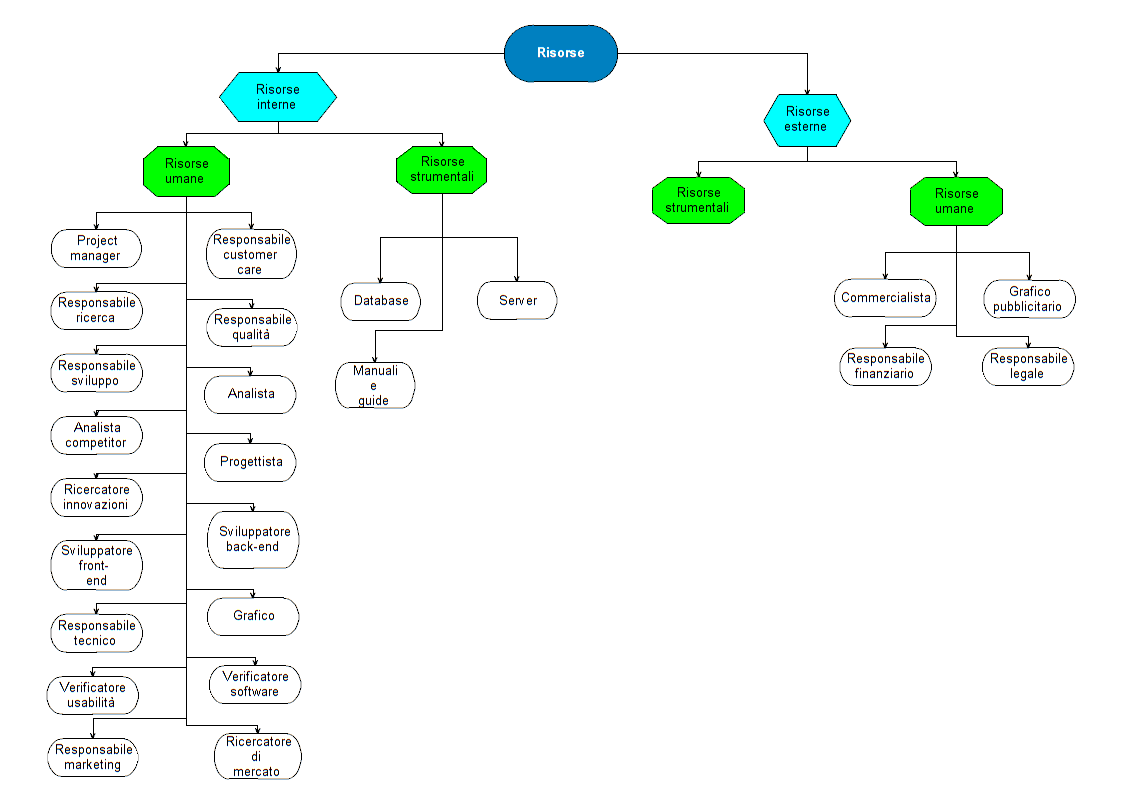
\includegraphics[scale=0.4]{img/Risorse_rbs.png}
\caption{Grafico RBS}
\label{fig:Grafico RBS}
\end{figure}
